\documentclass[a4paper,12pt]{report}

\usepackage[french]{babel}
\usepackage{geometry}
\usepackage[utf8]{inputenc}
\usepackage{listings}
\usepackage{graphicx}
\usepackage{color}
\usepackage{libertine}
\usepackage{amsmath}
\usepackage{amssymb}

\date{\today}

\geometry{hmargin=2cm,vmargin=3cm}

\def\D{\displaystyle} 

\lstdefinestyle{Python}{%
frame=single,
xleftmargin=2em,
language=python,
numbers=left,
numberstyle=\footnotesize,
columns=[l]flexible,
tabsize=3,
showtabs=true,
tab=$\color{gris!70}\to$,% \rightarrowfill,
backgroundcolor=\color{paille!15},
stringstyle=\color{gris}\
itshape,
showstringspaces=false,
keywordstyle=\color{broudenoix}\ttfamily,
commentstyle=\color{vertavocat}\itshape,
% mot des bibliotheques
emph={open,split,readlines,close,append,isdir,groups,Win32_LogicalDisk,argv,match,
VolumeName,showinfo,len},
emphstyle=\color{chocolat}\ttfamily,
% import usuels
emph={[2]os,sys,time,re,shutil,wmi,glob,tkMessageBox,path,tkm},
emphstyle={[2]\color{brun}\ttfamily\itshape},
}


\begin{document}
\lstset{
  language=Python,
} 


\begin{titlepage}
  \begin{sffamily}
  \begin{center}

    % Upper part of the page. The '~' is needed because \\
    % only works if a paragraph has started.
    
\includegraphics[scale=0.3]{ensl.jpg}~\\[1.5cm]

    \textsc{\LARGE École Normale Supérieur de Lyon}\\[2cm]

    \textsc{\Large Rapport de stage L3}\\[1.5cm]

    % Title
    { \huge \bfseries Outis pour l'analyse de grands systèmes aléatoires\\[1cm] }

    
\includegraphics[scale=0.6]{logo-uga.png}
    \\[2cm]

    % Author and supervisor
    \begin{minipage}[m]{0.55\textwidth}
      \begin{flushleft} \large
        Emmanuel \textsc{Rodriguez}\\
        Informatique théorique \\
        Promo 2016-2017\\
      \end{flushleft}
    \end{minipage}
    \begin{minipage}[m]{0.35\textwidth}
      \begin{flushright} \large
        \emph{Tuteur :} M. Nicolas \textsc{Gast}\\
        \emph{Co-encadrante :} Mme Florence \textsc{Perronnin}\\
        \emph{Chef d'équipe :} M.Arnaud \textsc{Legrand} \\
        \emph{équipe : } \textsc{POLARIS}
      \end{flushright}
    \end{minipage}

    \vfill

    % Bottom of the page
    {\large 29 Mai 2017 — 10 Juillet 2017}

  \end{center}
  \end{sffamily}
\end{titlepage}


\tableofcontents

\chapter*{Remerciements}

Je tiens à remercier toutes les personnes qui ont contribué au succès de mon stage et qui m'ont aidées lors de la rédaction de ce rapport.

Tout d'abord, je tiens à remercier vivement mon maître de stage, M.
Nicolas \textsc{Gast}, et Mme Florence \textsc{Perronnin} co-encadrante du stage, pour leur accueil, le temps passé ensemble et le partage de leur expertise au quotidien. Grâce aussi à leur confiance j'ai pu m'accomplir totalement dans mes missions. Ce fut une aide précieuse dans les moments les plus délicats.

Je remercie également toute l'équipe \textsc{POLARIS} pour son
accueil  et tous les bons moments passés ensemble.

Enfin, je tiens à remercier toutes les personnes qui m'ont conseillé
et relu lors de la rédaction de ce rapport de stage : ma famille, mon
ami Vincent \textsc{Rébiscoul} pour avoir partagé le même bureau de stage.


\chapter*{Introduction}
\addcontentsline{toc}{chapter}{Introduction}

On utilise des systèmes aléatoires dans de nombreux domaines de
l'informatique comme les réseaux de communication,les systèmes
distribués ou les systèmes de calcul... Ces systèmes, utilisés pour étudier
et améliorer la performance algorithmique distribuée, sont souvent
composés de nombreux objets en interaction, ce qui rend leur analyse
exacte difficile. \\
\smallbreak
Nous nous intéresserons dans ce stage à des outils
stochiastiques permettant de montrer que pour de nombreux systèmes, la
performance d'un système composé de N objets a une limite quand N est grand. \\
Plus précisément on s'intéressera au cours de ce stage aux chaines de Markov à temps
continu, un modèle pouvant s'appliquer à de nombreux problèmes allant
de la répartition des tâches dans un réseau à la répartition des vélos
dans les systèmes Vélo'v d'une ville. Nous établierons dans un
premier temps des outils de calcul s'appliquant à ces systèmes. Un
des objectifs principaux de ce stage sera d'implémenter une
bibliothèque \texttt{python3} générique permettant à l'utilisateur de
faire des simulations et des calculs sur ces chaînes de Markov à temps
continu. De plus cette bibliothèque nous permettra de valider le modèle
mis en place précédemment.

\chapter{Processus de population et bases théoriques}

\section{Chaîne de Markov à temps continu}

\paragraph{Lois exponentielles :} 
Une variable aléatoire $\D T \ $ à valeurs dans $\D \mathbb{R}_+ \ $ suit la
loi exponentiele de paramètre $\D \lambda \geq 0$, si  sa fonction de
répartition est donnée par $\D F(t)=(1-e^{-\lambda t})$ sur
$\D \mathbb{R}_+$. (et F(t)=0 sur $\D \mathbb{R}_-^*$).

\paragraph{}
Un \textbf{processus aléatoire} ou stochastique vise à décrire l’évolution généralement
temporelle (ou géométrique) d’une grandeur aléatoire. Formellement il s’agit
d’une famille $\D X = (X_{i} )\ i \in S$ de fonctions aléatoires $\D
X_{i}$ , à valeurs réelles, complexes ou vectorielles, sur un espace
de probabilité $\D (\Omega, F, P)$ et indicées par
un paramètre $\D i \in S\ $ où $\D S\ $ est un ensemble de référence.


\paragraph{Chaîne de Markov à temps continu :}

On considère un processus aléatoire $\D (X_t )_{t\in \mathbb{R}^+}$, à
valeurs dans un ensemble $\D E$ fini ou dénombrable ayant
la propriété suivante, appelée propriété de Markov : \\
pour tous $\D n \in N,\ 0 \leq t_0 < \ldots < t_{n+1}\ et\ x = x_0 ,
\cdots , x_n , x_{n+1}\ \in
E$

\begin{eqnarray*}
P(X_{t_{n+1}} = x_{n+1} \|X_{t_0} = x_0 ,\ldots , X_{t_n} = x_n ) &=& P(X_{t_{n+1}} = x_{n+1} \|X_{t_n} = x_n )
\end{eqnarray*}
lorsque l’événement $\D \{X_{t_0} = x_0 , \ldots , X_{t_n} = x_n \}$ est de probabilité non nulle.
Le processus $\D (X_t )\ t\in \mathbb{R}^+$ est alors appelé chaîne de Markov (continue).
Si $\D P(X_{t+s} = y \|X_t = x) = p_s (x, y)$ ne dépend pas de t, on dit
alors que $\D (X_t )\ t\in \mathbb{R}^+$
est une \textbf{chaîne de Markov à temps continu}(CMTC) ou \textbf{Processus de Markov à saut}.

L'un des principaux aspects de ce type de processus aléatoire est qu'il
est sans mémoire, l'avancement ne dépendant que de l'instant présent.


On pourra trouver de plus amples détails dans le document suivant \cite{courscmtc}.

\section{Processus de population}
Nous reprendrons le modèle  établi par Kurtz \cite{kurtz}. Soit
$\D (X^{(N)})$ une CMTC. $\D X^{(N)}\ $ représente la
\textbf{proportion de population} de chaque état. Il existe $\D L \in
\epsilon$, avec $\D n=card(S)\ $et $\D \epsilon\ $ un ensemble borné de
$\D \mathbb{R}\ $,
et un ensemble de fonctions $\D \beta_l^{(N)}: \epsilon \rightarrow
\mathbb{R}^+$ tel que $\D X^{(N)}\ $ passe de l'état $\D x\ $ à
l'état $\D x+\frac{l}{N}\ $ avec le taux $\D N\beta_l^{(N)}\ $ pour
tout $\D l\in L$.

On définit alors le drift:
\begin{eqnarray*}
  \D f^{(N)}(x)=\sum_{l\in L}l\beta_l^{(N)}(x)
\end{eqnarray*}

Le drift représente l'avancement infinitésimal du système. 

\section{Approximations}

Nous supposerons dans le cadre de ce stage les propositions suivantes:
\begin{itemize}
\item  $\D sup_{x\in \epsilon,N \geq 1}\sum_{l\in
    L}\beta_l^{(N)}\|l\|^2 \ < \ \infty$
\item  $\D f^{(N)}(x) \ =\  f(x)+\frac{\tilde{f}(x)}{N}+O(\frac{1}{N^2}) $
\item  $f$ est deux fois dérivable et $\D\ddot{f}\ $est uniformément continue et bornée.
\item  $\D \dot{x}=f(x)$ possède un unique attracteur $\pi$ exponentiellement stable.
\end{itemize}

\paragraph{Théorème} \cite{approx} Soit $\D h: \epsilon \rightarrow \mathbb{R}^+\ $
deux fois dérivable et dont la dérivée seconde est uniformément
continue. Alors:
\begin{eqnarray*}
  \lim_{N \rightarrow \infty}N\left(
  E^{(N)}\left[h(X^{(N)})\right]-h(\pi)\right)
  &=&
      \sum_i \frac{\partial h}{\partial x_i}(\pi)D_i + \frac{1}{2}
      \sum_{i,j} \frac{\partial^2h}{\partial x_i \partial x_j}(\pi)W_{ij}
\end{eqnarray*}

Avec:
\begin{itemize}
\item $\D A_{i,j}= \frac{\partial f_i}{\partial x_j}(\pi)$
\item $\D (B_j)_{k_1,k_2}=\frac{\partial^2f_j}{\partial
    x_{k_1} \partial x_{k_2}}(\pi)$
\item $W \ $ l'unique solution de l'équation de Lyapunov suivante $\D
  AW+WA^T+Q=0$
\item $\D D_i=-\sum_j(A^{-1})_{i,j}\left[ C_j+\frac{1}{2}\sum_{k_1,k_2}(B_j)_{k_1,k_2}W_{k_1,k_2}\right]$
\end{itemize}

On a donc $\D X_i^{(N)}=\pi_i+\frac{D_i}{N}+o(\frac{1}{N})\ $ lorsque N
tend vers l'infini.

\paragraph{}
On cherchera par la suite à calculer ce coefficient $\D D_i\ $ à
l'aide du théorème et a vériffier sa validité en calculant ce
coefficient par simulation.

\chapter{Réalisation d'une bibliothèque générique}

Pour vérifier le modèle étudié j'ai codé une bibliothèque \cite{librairie} dans le
langage \texttt{python3} qui permet de simuler une CMTC et de calculer le
coefficient en $\D \frac{1}{N}$, pour une CMTC quelconque.

\section{Le simulateur}

\subsection{Réalisation}
Pour la simulation, nous suivons le schéma suivant :

\begin{itemize}
\item recherche de la prochaine transition
\item effectuer cette transition
\item recommencer tant qu'on a pas atteint le temps limite
\end{itemize}



\paragraph{Méthode naive :}

Soit $\D l \in L \ $ un vecteur représentant une transition. Cette
transition est associée au taux $\D \beta_l \ $. Le système passe d'un
état $\D X \ $ à $\D X+\frac{l}{N} \ $ avec le taux $\D N*\beta_l \ $. On tire
la variable aléatoire  $\D expo(N*\beta_l) \ $ pour obtenir le temps avant cette transition. Avec expo(i) une
loi exponentielle de paramètre i. On tire donc une loi exponentielle
pour chaque transition puis seule la transition qui a lieu en premier est
prise en compte. \\

Mais il existe  une méthode plus rapide et équivalente:

\paragraph{Amélioration :}


Pour savoir quelle transition aura lieu en premier, on peut plus
simplement choisir une transition $\D l$ avec proba:
$\D \frac{\beta_l}{\sum_{i \in L}\beta_i}$, en tirant juste un réel entre 0 et 1 par exemple.
Puis une fois la transition choisie on tire une loi exponentielle de
paramètre $\D \sum_{i \in L}\beta_i$ pour obtenir le temps avant la
transition.


\paragraph{Réalisation d'un simulateur} 

J'ai codé en \texttt{python3} le simulateur suivant prenant en entrée une chaîne
de Markov a temps continu quelconque. La fonction comprend deux
options qui sont les deux dernier arguments : on peut fixer la graine
qui sert à générer l'aléatoire du module random de \texttt{python3}. Ce qui
sert à pouvoir refaire la même simulation avec exactement les mêmes
conditions. (Il faut alors ajouter l'argument: $\D fix=1234$ par exemple)

La seconde option permet d'écrire dans un fichier (dont on
précise le nom avec l'argument : $\D file=''mon\_fichier.out''$) le tableau
de données représentant la simulation effectuée.

La simulation renvoie un doublet \texttt{data}:
\begin{itemize}
\item \texttt{data[0]} le tableau des temps
\item \texttt{data[1]} la matrice des valeurs des $\D X_i$ aux
  différents temps
\end{itemize}

\subsection{Exemple d'utilisation: système d'infection SIR}
On considère le système suivant:

\begin{eqnarray}
  S & \rightarrow & I \ \ taux \  = \  3x_0x_1+\frac{x_0}{2}\\
  I & \rightarrow & R \ \ taux \ = \ x_1\\
  I+R & \rightarrow & S \ \ taux \ = \ 2x_1x_2 
\end{eqnarray}

On note $\D X=\left[ x_1;x_2;x_3\right]$ les proportions de S I R:
\begin{eqnarray*}
  x_0 &=& \frac{population(S)}{population\ totale} \\
  x_1 &=& \frac{population(I)}{population\ totale} \\
  x_2 &=& \frac{population(R)}{population\ totale}
\end{eqnarray*}

On simule cet exemple de la façon suivante avec le simulateur codé
précédemment avec comme condition initiale $\D X_0=\left[\frac{1}{2};\frac{1}{2};0\right]$ \\
\newpage
\begin{lstlisting}[frame=single]
  liste_transitions = [ array(l) for l in [ [-1.,+1.,0.], [0.,-1.,1.],
  [2.,-1.,-1.] ] ]

  def taux ( i, x):
     if i==0:
        return 3*x[0]*x[1]+0.5*x[0]
    elif i==1:
        return x[1]
    else:
        return 2*x[1]*x[2]
    
  labels=["S","I","R"]
  X=array([0.5,0.5,0.])

  simu_cmtc(taux,liste_transitions,X,1000,20,"data.out",1234)

  data=file_to_array("data.out",3)

  for i in range(3):
    plot(data[0],data[1][:,i], label=labels[i])

  legend()
  show()
\end{lstlisting}

\begin{center}
  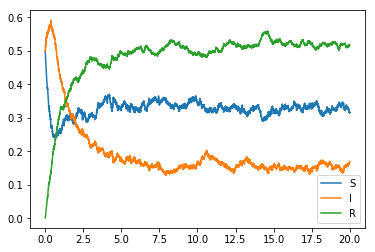
\includegraphics{figure1.png}
\end{center}

On obtient bien un résultat qui paraît cohérent au premier coup
d'\oe il. Pour vérifier cette simulation on résout l'équation
différentielle qui régit ce système:

\begin{eqnarray*}
  \dot{x} &=& f(x)
\end{eqnarray*}

La bibliothèque contient une fonction $print\_simu$ qui nous permet de tracer sur la même courbe la
simulation et la solution théorique du système.
Avec les quelques lignes de code suivantes on obtient:

\begin{lstlisting}[frame=single]
  print_simu(taux,liste_transitions,X,1000,20)
\end{lstlisting}

\begin{center}
  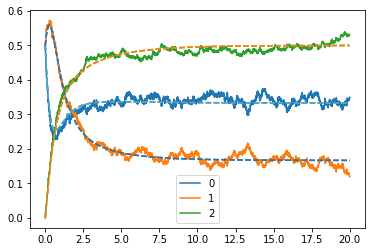
\includegraphics{figure2.png}
\end{center}

On a donc la confirmation que pour ce système la simulation est
cohérente avec le résultat théorique. (L'ordre de grandeur et le signe
sont équivalents).

\section{Calcul du coefficient en $1/N$}

\subsection{Par simulation}

Pour calculer le coefficient en 1/N, on fait la moyenne des
points fixes obtenus lors de n simulations, à laquelle on soustrait le point fixe calculé théoriquement: $\D C =
\frac{\sum_{i=0}^{n-1}{E(X^{(N)}_i)}}{n}-X_0 \ $

Pour calculer le point fixe par simulation on fait une moyenne sur le
dernier tiers des termes d'une simulation longue (assez longue pour
qu'on atteigne largement le point fixe).

\paragraph{Remarque}
Le choix de la longueur de la simulation pour qu'on atteigne largement
le point fixe est purement arbitraire. \\

Mais le résultat de $\D C \ $ ne correspond pas ! Un autre terme d'erreur en
$\D O(\frac{1}{N})$ est apparu lors du calcul des points fixes par
simulation. La moyenne calculée des termes de la simulation ne prend
pas en compte le temps entre chaque transition d'où ce terme en
$\D O(\frac{1}{N})$.

Pour y remédier on calcule une moyenne pondérée par le temps entre
chaque transition.

Afin de valider ce modèle, on lance le calcul du coefficient sur un
grand nombre de simulations et pour des valeurs différentes de N. On
trace sur la courbe ci-dessous la moyenne de 100 simulations par point
pour atténuer les perturbations dûes à l'aléatoire. Pour
chaque simulation le coefficient doit être identique.

\begin{lstlisting}[frame=single]
  N=linspace(10,1000,20)
  diff=array([[0. for i in N] for j in range(3)])
  C_i=array([[0. for i in N] for j in range(3)])
  X_0=fixed_point(taux,liste_transitions,3)

  for n in range(len(N)):
    for j in range(100):
      data=simu_cmtc(taux,liste_transitions,X,N[n],50)
        for i in range(3):
        diff[i,n]+=(moy_pond(data,int(len(data[1])/2),
                    len(data[1]),i)-X_0[i])/100.
    for i in range(3):
      C_i[i,n]=N[n]*diff[i,n]

  for i in range(3):
    plot(N,C_i[i,:])
  legend(('S','I','R'))
  show()
\end{lstlisting}

On obtient alors:
\begin{center}
  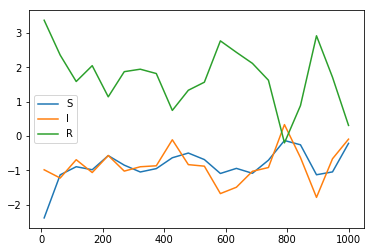
\includegraphics{figure3.png}
\end{center}

On observe un bruit important pour les grandes valeurs de N, ce qui est
sûrement dû aux erreurs de calcul sur les réels avec \texttt{python3}. On
observe donc $\D x_s=-1 \ x_I=-1\ x_R=2$ avec un bruit important pour 100
simulations par point. Le temps de calcul pour ce résultat est
d'environ 40 minutes (avec un code non optimisé).

\subsection{Validation à l'aide du calcul théorique de ce coefficient}
On a montré que le coefficient d'erreur en $\D \frac{1}{N} \ $ vaut
exactement:

\begin{eqnarray*}
  D_i=\frac{1}{2}*\sum_{j}((A^{-1})_{i,j}*\sum_{k_1,k_2}(B_j)_{k_1,k_2}W_{k_1,k_2})
\end{eqnarray*}

Avec:
\begin{itemize}
\item $\D A_{i,j}=Df(x^*)_{i,j}$
\item $\D (B_j)_{k,l}=$
\item $\D W \ $ est la solution de l'équation de Lyapunov suivante: $\D AX+XA^T+Q=0$
\item $\D Q=\sum_{l \in L} Q_l$
\item $\D (Q_l)_{n,m}=-l_nl_m \beta_l(x^*)$
\end{itemize}

L'implémentation de ce calcul est réalisée à l'aide du module de
calcul symbolique de \texttt{python3} (Annexe A).

Cette fonction nous permet donc de calculer le coefficient de manière
théorique. Mais les systèmes étudiés ont souvent cette équation de
vérifié :
\begin{eqnarray*}
  \sum_{x \in X}x &=& 1
\end{eqnarray*}
Le système SIR par exemple vérifie $\D x_S+x_I+x_R=1$. On étudie alors n
systèmes de dimention 2 et non 3. Il faut donc le préciser à l'entrée
de la fonction: $\D n=3 \ et \ dim=2$.

\begin{lstlisting}[frame=single]
  theorique(taux,liste_transitions,3,2)
\end{lstlisting}

On obtient: $\D D_S=-0.75000000000000111,\ D_I=-0.96428571428571352$ 
ce qui correspond bien aux valeurs calculées par simulation. On peut
en déduire $\D D_R=1-D_S-D_I$.  Ce calcul
n'a pris que quelques secondes à calculer, comparé aux 40 minutes du
résultat approximatif des simulations.

Pour un exemple simple comme le système SIR, on a déjà des problèmes de
temps de calcul par simulation. La formule précédente facilite donc
grandement le calcul du coefficient en 1/N.


\chapter{Résultats expérimentaux}
\section{Modèle d'infection SIR}
L'exemple est détaillé dans le chapitre précédent. Il permet de
valider pour cet exemple simple le modèle étudié.

\section{Bianchi's formula}
On s'interésse ici à un modèle \cite{bianchi} pour le protocole 802.11 MAC. On le
modélise à l'aide d'une chaine de Markov. On obtient la CMTC aux transitions suivantes:

\begin{eqnarray*}
  x & \rightarrow & x+e_0-e_k \ avec\ un\ taux \
  q_kx_k\prod_{m=0}^K(1-\frac{q_m}{N})^{Nx_m-e_k} \ for \ k \in
                    \{1...K-1\} \\
  x & \rightarrow & x+e_{k+1}-e_k \ avec\ un\ taux \
  q_kx_k(1-\prod_{m=0}^K(1-\frac{q_m}{N})^{Nx_m-e_k}) \ for \ k \in
                    \{1...K-1\} \\
  x & \rightarrow & x+e_0-e_K \ avec \ un \ taux \ q_Kx_K
\end{eqnarray*}

On entre alors le système de la manière suivante dans notre
simulateur:

\newpage
\begin{lstlisting}[frame=single]
N=100
K=5
Var_x=array([sym.symbols('x_{}'.format(i)) for i in range(K)])
#Var_q=array([sym.symbols('q_{}'.format(i)) for i in range(K)])
Var_q=array([2**(-i) for i in range(K)])

def mult_liste(Liste):
    S=1
    for i in Liste:
        S*=i
    return(S)

E=[array([1 if i==j else 0 for j in range(K)]) for i in range(K)]

liste_transitions =[]
taux=[]

liste_transitions.append(E[1]-E[0])
taux.append(Var_q[0]*Var_x[0]*
(1-mult_liste([(1-Var_q[m]/N)**(N*Var_x[m]-(0 if m!=0 else 1)) 
                                            for m in range(K)])))

for i in range(1,K-1):
    liste_transitions.append(E[0]-E[i])
    taux.append(Var_q[i]*Var_x[i]*
    mult_liste([(1-Var_q[m]/N)**(N*Var_x[m]-(0 if m!=i else 1)) 
                                              for m in range(K)]))
    liste_transitions.append(E[i+1]-E[i])
    taux.append(Var_q[i]*Var_x[i]*
    (1-mult_liste([(1-Var_q[m]/N)**(N*Var_x[m]-(0 if m!=i else 1)) 
                                                 for m in range(K)])))

liste_transitions.append(E[0]-E[K-1])
taux.append(Var_q[K-1]*Var_x[K-1])

def fct_taux(i,X):
    return sym.lambdify( Var_x,taux[i])(*X)
\end{lstlisting}

Puis on entre les conditions initiales et on trace le tout :

\begin{lstlisting}[frame=single]
X=[1/K for i in range(K)]
print_simu(fct_taux,liste_transitions,X,1000,15)
\end{lstlisting}

On obtient la figure suivante :

\begin{center}
  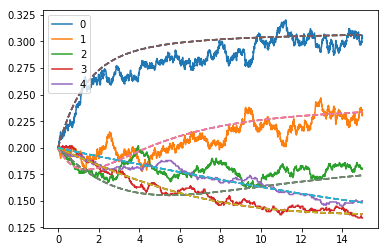
\includegraphics{bianchi.png}
\end{center}
  
Le tracé suit bien la solution de l'équation différentielle qui régit
le système. Un simple tracé comme celui-ci met déjà quelques minutes à
se faire. Le calcul du coefficient recherché en 1/N est trop long à
calculer avec des simulations. Car il nous faudrait un grand nombre de
simulations pour obtenir un résultat exploitable.

\begin{lstlisting}[frame=single]
theorique(fct_taux,liste_transitions,5,4)
\end{lstlisting}

Le calcul à l'aide de la formule se fait en quelques minutes et on
obtient :  $\D  D_0=-0.038851395750410606,\ D_1= 0.075038237961333909,\
  D_2=0.037170741481473424,\ D_3= -0.016174636251891139 $ 

Ce système converge donc rapidement car les coefficients sont de
l'ordre de $\D 10^{-2}$.

\section{Vélo'v}
La répartition et l'évolution du nombre de vélos par station de Vélo'v
peut facilement se modéliser avec une chaîne de Markov. On peut utiliser
un tel modèle décrit dans de document: \cite{velov} pour optimiser le nombre de vélos par station par
exemple.
On entre cette CMTC de la manière suivante dans le simulateur:

\newpage
\begin{lstlisting}[frame=single]
K=10
N=20
s=3
Lambda=1
Mu=0.5

y=array([sym.symbols('y_{}'.format(i)) for i in range(K)])
E=[array([1 if i==j else 0 for j in range(K)]) for i in range(K)]
liste_transition=[]
taux=[]

for i in range(K-1):
    liste_transition.append(E[i+1]-E[i])
    taux.append(Mu*y[i]*(s-sum([n*y[n] for n in range(K)])))
    
for i in range(1,K):
    liste_transition.append(E[i-1]-E[i])
    taux.append(Lambda*y[i])
    
def fct_taux(i,X):
    return(sym.lambdify(y,taux[i])(*X))
\end{lstlisting}

Il ne nous reste plus qu'à choisir une distribution initiale et à tracer
l'évolution.

\begin{lstlisting}[frame=single]
X=[1,0,0,0,0,0,0,0,0,0]
print_simu(fct_taux,liste_transition,X,100,10)
\end{lstlisting}

On obtient alors la courbe suivante :

\begin{center}
  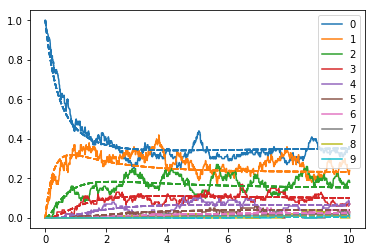
\includegraphics{velov.png}
\end{center}

\newpage
\begin{lstlisting}[frame=single]
X=[1,0,0,0,0,0,0,0,0,0]
theorique(fct_taux,liste_transition,K,K-1)
\end{lstlisting}

On obtient alors: \\
$\D D_0=-0.10292176084411847$, \\
$\D D_1=0.039044474621688807$, \\
$\D D_2=0.064763975313775535$,\\
$\D D_3=0.048762058614485009$,\\
$\D D_4=0.023866044952782651$,\\
$\D D_5=0.002612691487885844$,\\
$\D D_6=-0.01170356394907981$,\\
$\D D_7=-0.019540234122908881$,\\
$\D D_8=-0.022526472856673283$ 

 On obtient un coefficient de l'ordre du centième, ce qui est
 relativement faible. Le système converge donc très rapidement.


\chapter{Organisation du stage}
\section{Projet GitHub}
 Le travail effectué pendant la durée du stage est contenu dans un
 projet GitHub\cite{librairie} contenant:
\subsection{Bibliothèque \texttt{python3}}
L'ensemble du code est rassemblé dans une bibliothèque \texttt{python3}
 qui
contient les fonctions suivantes dont l'utilisation est détaillée précédemment:
\begin{itemize}
  \item
    $\D simu\_ctmc(fct\_taux,liste\_transition,X_0,N,temps\_final,'mon\_fichier.out',fix\_seed)
    \ $
     simule notre CMTC.
  \item $\D file\_to\_array('mon\_fichier.out',len(X)) \ $  permet de
    récupérer les données que l'on a précédemment stockées dans un
    fichier.
  \item $\D fixed\_point(taux,liste\_transition,n) \ $  renvoie un vecteur
    des points fixes du système calculé à l'aide de la
    \texttt{odeint} de \texttt{python3}.
  \item $\D theorique(taux,liste_transition,n,dim)$  calcule le
    coefficient d'erreur en $\D 1/N \ $ de manière théorique.
\end{itemize}

\subsection{Notebook d'exemples}
Ce fichier \texttt{ipython} contient les exemples étudiés pendant le stage et
peut donc servir de notice pour l'utilisation du simulateur et des
autres fonctions de calcul. 

\section{Outils utilisés}

\subsection{Ubuntu 17.04}
Le travail a été effectué sous la version 17.04 d'Ubuntu. Les commandes
d'installation fournies ci-dessous fonctionnent avec un système Debiane à jour.

\subsection{Org-mode dans emacs}
Au cours de ce stage j'ai découvert org, un modude que l'on peut
greffer à emacs, qui sert à écrire un journal de bord de manière simple
et propre. Cet outil permet entre autre de générer un pdf propre du
journal de bord, d'y lier des fichiers, des réferences... Cet outil
est très riche et permet donc un suivi du travail efficace.
\begin{verbatim}
sudo apt-get install emacs25 org-mode ess r-base auctex
\end{verbatim}

\subsection{Jupyter-notebook}
Le notebook Jupyter est une façon simple et lisible de
coder en \texttt{python3} à l'aide des fichiers \texttt{ipython} qui
sont de la programmation littérale. Cet outil permet d'exécuter
des parties de code rapidement et indépendemment des autres. Ainsi que
de glisser des commentaires de façon propre et rapide. Le fichier
\texttt{ipython} conserve aussi les sorties renvoyées par le code comme les
graphiques et autres.

\begin{verbatim}
sudo apt-get install jupiter-notebook ipython3 ipython3-notebook
\end{verbatim}

\subsection{Bibliothèque \texttt{python3}}
Dans le code écrit, j'utilise les fonctions suivantes de \texttt{python3}:
\begin{lstlisting}[frame=single]
from random import random,seed,expovariate
from pylab import array
from numpy import linspace,zeros
from matplotlib.pyplot import *
import sympy as sym
from scipy.integrate import odeint
from scipy.linalg import solve_lyapunov
from numpy.linalg import inv
\end{lstlisting}

Il est alors nécessaire de les installer précédemment pour pouvoir
utiliser la bibliothèque.

\begin{verbatim}
sudo apt-get install python3-random python3-pylab python3-numpy
python3-matplotlib python3-sympy python3-scipy 
\end{verbatim}


\chapter*{Conclusion}
\addcontentsline{toc}{chapter}{Conclusion}

Au cours de ce stage nous avons codé une bibliothèque générique
\texttt{python3} qui nous a permi d'une part à valider certains
résultats étudiés au cours de ce stage et d'autre part à montrer que
le calcul de la constante  $\D D_i$, nous permetant d'optimiser les
systèmes étudiés et à mieux les comprendre, est laborieux par
simulation. Alors que ce calcul peut s'effectuer de manière plus
rapide, pour les exemples étudiés, à l'aide du théorème provenant des
travaux de Nicolas \textsc{Gast}.
Les outils développés au cours de ce stage ont été conçus pour être
génériques et faciles d'utilisations. Pouvant ainsi être réutilisés
sans trop de difficultés pour des recherches futures.



\appendix

\chapter{Bibliothèque python3}
\label{biblip3}
\begin{lstlisting}[frame=single]
from random import random,seed,expovariate
from pylab import array
from numpy import linspace,zeros
from matplotlib.pyplot import *
import sympy as sym
from scipy.integrate import odeint
from scipy.linalg import solve_lyapunov
from numpy.linalg import inv


def simu_cmtc(taux,L,X,N,time,file="",fix=-1):
    n=len(X)
    nb_trans=len(L)
    t=0
    
    if fix!=-1:
        seed(fix)

    if file!="":
        data=open(file,"w")
    else:
        data=[[0],[X]]
        
    while t<time:
        a=random()
        
        L_poids=array([taux(i,X) for i in range(nb_trans)])
        S=sum(L_poids)
        
        cumul=0
        for i in range(nb_trans):
            tmp=cumul + L_poids[i]/S
            if a < tmp:
                l=i
                break
            cumul=tmp
        
        X = X+(1./N)*L[l]
        if max(L_poids)==0:
            break

        expo=expovariate(N*S)
        t+=expo

        if file=="":
            data[0].append(t)
            data[1].append(X[:])
        else:
            data.write(str(t)+" ")
            
            for i in range(n):
                data.write(str(X[i])+" ")
            data.write('\n')
    
    if file=="":
        data[1] = array(data[1])
        return(data)
    else:
        data.close()
        return(0)


def file_to_array(file,n):
    fichier=open(file,"r")
    texte=fichier.read()
    
    tmp=texte.split( )
    tmp=[tmp[i].split(' ',1) for i in range(len(tmp))]
    data=[[],[]]
    for i in range(int(len(tmp)/(n+1))):
        data[0].append(float(tmp[i*(n+1)][0]))
        data[1].append([float(x[0]) for x in tmp[i*(n+1)+1:i*(n+1)+n+1]])
    data[1]=array(data[1])
    return(data)



def fixed_point(taux,liste_transitions,n):
    number_transitions = len(liste_transitions)    
    def drift(x):
        return (sum([liste_transitions[i]*taux(i,x)
                     for i in range(number_transitions)],0))
    
    X0 = zeros(n)
    X0[0] = 1
    t = linspace(0,1000,1000)
    x = odeint( lambda x,t : drift(x), X0, t)
    #figure()
    #plot(x)
    #show()
    return(x[-1,:])


def theorique(taux,liste_transitions,n,dim):
    number_transitions = len(liste_transitions)  
    X_0 = fixed_point(taux,liste_transitions,n)
    
    Var=array([sym.symbols('x_{}'.format(i)) for i in range(n)])
    
    #print(len(X_0))
    f_x=array([0 for i in range(n)])
    for i in range(number_transitions):
        f_x = f_x + liste_transitions[i]*taux(i,Var)

    if dim==n-1:
        for i in range(n):
            f_x[i]=f_x[i].subs(Var[-1],1-sum(array([Var[i] 
                                                for i in range(n-1)])))

    A=array([[sym.lambdify(Var ,sym.diff(f_x[i],Var[j]))(*[X_0[k] 
                for k in range(n)]) 
              for j in range(dim)] 
             for i in range(dim)])

    B=array([[[sym.lambdify(Var,sym.diff(f_x[j],Var[k],Var[l]))
(*[X_0[i] for i in range(n)]) 
               for l in range(dim)] 
              for k in range(dim)] 
             for j in range(dim)])

    Q=array([[0. for i in range(dim)] for j in range(dim)])

    for l in range(number_transitions):
        Q += array([[liste_transitions[l][p]*liste_transitions[l][m]
*taux(l,X_0) 
                     for m in range(dim)] 
                    for p in range(dim)])


    
    W = solve_lyapunov(A,Q)

    A_inv=inv(A)
    
    C=[ 0.5*sum([A_inv[i][j]*sum(array([[B[j][k_1][k_2]*W[k_1][k_2] 
                                         for k_2 in range(dim)] 
                                        for k_1 in range(dim)])) 
                 for j in range(dim)]) 
       for i in range(dim)]
    for i in range(len(C)):
        C[i]=sum(C[i])
    return(C)

def print_simu(taux,liste_transition,X,N,time,fix=-1):
    data=simu_cmtc(taux,liste_transition,X,N,time,"",fix)
    K=len(X)
    for i in range(K):
        plot(data[0],data[1][:,i],label=str(i))
    def drift(x):
        return (sum([liste_transition[i]*taux(i,x)
                     for i in range(len(liste_transition))],0))
    
    t = linspace(0,time,1000)

    for i in range(K):
        x = odeint( lambda x,t : drift(x), X, t)
        plot(t,x,'--')
    legend()
    show()
\end{lstlisting}

\bibliographystyle{plain}
\bibliography{bibli}

\end{document}
